%% Run LaTeX on this file several times to get Table of Contents,\
%% cross-references, and citations.

\documentclass[11pt]{book}
\usepackage{Wiley-AuthoringTemplate}
\usepackage[sectionbib,authoryear]{natbib}
% for name-date citation comment the below line
%\usepackage[sectionbib,numbers]{natbib}% for numbered citation comment the above line

%%********************************************************************%%
%%       How many levels of section head would you like numbered?     %%
%% 0= no section numbers, 1= section, 2= subsection, 3= subsubsection %%
\setcounter{secnumdepth}{3}
%%********************************************************************%%
%%**********************************************************************%%
%%     How many levels of section head would you like to appear in the  %%
%%				Table of Contents?			%%
%% 0= chapter, 1= section, 2= subsection, 3= subsubsection titles.	%%
\setcounter{tocdepth}{2}
%%**********************************************************************%%

%\includeonly{ch01}
\makeindex
\usepackage{pdfpages}

\newcommand{\upRiemannint}[2]{
  \overline{\int_{#1}^{#2}}
}
\newcommand{\loRiemannint}[2]{
  \underline{\int_{#1}^{#2}}
}

\usepackage[T1]{fontenc}
%\usepackage{mathrsfs}
\graphicspath{{picture/}}


%\includeonly{chapter/chapter3/chapter3}


\begin{document}

\frontmatter
%%%%%%%%%%%%%%%%%%%%%%%%%%%%%%%%%%%%%%%%%%%%%%%%%%%%%%%%
%% Setting up title pages, type in the appropriate names here:
\booktitle{Analysis \uppercase\expandafter{\romannumeral2} Manual Script}

%\subtitle{}

\AuAff{
Xinhao Yang\\ The Chinese University of Hongkong, Shenzhen}

%% Print Half Title and Title Page:
%\halftitlepage
\titlepage


%%%%%%%%%%%%%%%%%%%%%%%%%%%%%%%%%%%%%%%%%%%%%%%%%%%%%%%%
%% Only Dedication (optional) 
\dedication{Read the masters!}


\tableofcontents

%%%%%%%%%%%%%%%%%%%%%%%%%%%%%%%%%%%%%%%%%%%%%%%%%%%%%%%%
% Optional Preface:
\begin{preface}
As Terence says in his book, students should write down every step of each excercise instead of ``cheating''. Taking his advice, here comes the book. However, it's too time consuming to write down every single step with \LaTeX. Considering this, I will only type critical steps and significant tricks towards excercises that worth my time.\\The book is written as a notebook for myself which means there may exists many oral expressions or feelins of myself. If , oneday, the book is read by some of my friends, please ignore those personal words. Also, I writing this book to learn how to write rigorously without many grammer mistakes. If you use this book as a reference and encouter some of unclearly expressions or typos during reading, please contact Xinhao Yang at the first time.

\prefaceauthor{}
\where{CUHK(SZ)\\
 \today}
\end{preface}

%%%%%%%%%%%%%%%%%%%%%%%%%%%%%%%%%%%%%%%%%%%%%%%%%%%%%%%%
% Optional Acknowledgments:

\acknowledgments
The excercises which this book provided manual script for are from outstanding mathematician Terence Tao's book {\it Analysis \uppercase\expandafter{\romannumeral2}}.  
\\
Thank Pro. Yutian Li for his recommendation for such a brilliant book .
\\
Thank Jie Wang for his generous help in \LaTeX.
%\authorinitials{CUHK(SZ)}  


%%%%%%%%%%%%%%%%%%%%%%%%%%%%%%%%%%%%%%%%%%%%%%%%%%%%%%%%
% Optional notations:
\begin{notations}
\acro{$\mathbb{R}^n$}{$n$-dimensional real space}
\acro{$\mathbb{C}^n$}{$n$-dimensional complex space}
\acro{$\mathbb{R}^{m\times n}$}{set of all $m\times n$ real-valued matrices}
\acro{$\mathbb{C}^{m\times n}$}{set of all $m\times n$ complex-valued matrices}
\acro{$x_i$}{$i$th entry of column vector $\bm x$}
\acro{$a_{ij}$}{$(i,j)$th entry of matrix $\bm A$}
\acro{$\bm a_i$}{$i$th column of matrix $\bm A$}
\acro{$\bm a_i\trans$}{$i$th row of matrix $\bm A$}
\acro{$\mathbb{S}^n$}{set of all $n\times n$ real symmetric matrices, i.e., $\bm A\in\mathbb{R}^{n\times n}$ and $a_{ij}=a_{ji}$ for all $i,j$}
\acro{$\mathbb{H}^n$}{set of all $n\times n$ complex Hermitian matrices, i.e., $\bm A\in\mathbb{C}^{n\times n}$ and $\bar{a}_{ij}=a_{ji}$ for all $i,j$}
\acro{$\bm A\trans$}{transpose of $\bm A$, i.e, $\bm B=\bm A\trans$ means $b_{ji}=a_{ij}$ for all $i,j$}
\acro{$\bm A\Her$}{Hermitian transpose of $\bm A$, i.e, $\bm B=\bm A\Her$ means $b_{ji}=\bar{a}_{ij}$ for all $i,j$}
\acro{$\trace(\bm A)$}{sum of diagonal entries of square matrix $\bm A$}
\acro{$\bm 1$}{A vector with all $1$ entries}
\acro{$\bm 0$}{either a vector of all
zeros, or a matrix of all zeros}
\acro{$\bm e_i$}{a unit vector with the nonzero element at the $i$th entry}
\acro{$\mathcal{C}(\bm A)$}{the column space of $\bm A$}
\acro{$\mathcal{R}(\bm A)$}{the row space of $\bm A$}
\acro{$\mathcal{N}(\bm A)$}{the null space of $\bm A$}
\acro{$\Proj_{\mathcal{M}}(\bm A)$}{the projection of $\bm A$ onto the set $\mathcal{M}$}
\end{notations}
\mainmatter
\setcounter{page}{1}


\chapter{Metric spaces}
\section{Definitions and examples}
%create a math proof environment
	\paragraph{\it Excercise 1.1.1.}{\it Proof.} $\Rightarrow \forall\varepsilon \quad\exists N\quad\text{s.t.} \quad\forall n \geqslant N\quad |x_{n}-x| \leqslant\varepsilon$ which is to say $\diff (x_{n},x) \leqslant \varepsilon$. Therefore, $\lim_{n\rightarrow\infty}\diff(x_{n},x)=0$.\\
	
	$\Leftarrow \quad \forall\varepsilon \quad\exists N\quad\text{s.t.} \quad\forall n \geqslant N\quad \diff(x_{n},x)\leqslant\varepsilon $ which means $ |x_{n}-x| \leqslant\varepsilon$\\Therefore, $(x_{n})_{n=m}^{\infty}$ indeed converges to $x$.

\paragraph{\it Excercise 1.1.2.}

\paragraph{\it Excercise 1.1.3.}
\begin{itemize}
\item[(a)]d(x,y):=0.5(x=y),1(x$\neq$y)
\item[(b)]d(x,y):=0 (for any x,y$\in$X)
\item[(c)]X:=\{x,y,z\}  d(x,y):=0.5; d(y,x):=1;d(a,b):=1 (a$\neq$b).d(a,b):=0(a=b)
\item[(d)]Pick three point on a line makes X. Their distances in between be 1,1,3.

\end{itemize}


\paragraph{Excercise 1.1.4}
Firstly, the subset and restricted function all induced four properties or we say they satisfied four axioms automatically.

\paragraph{Excercise 1.1.5}
First equation use induction.
With the first equation, we can get second equation directly(remove the second part, positive, on the left hand side and then find square root of both sides).(see also linear algebra for a different proof)\\
With a little bit arrange( square the inequality and exchange finite summation symbol), we can get the final inequatlity.
\paragraph{Exercise 1.1.6}
Just get used to four axioms of being a metric space.With the help of third inequality in excercise1.1.5 for forth axiom.
\paragraph{Exercise 1.1.7.}
Nothing special.
\paragraph{Exercise 1.1.8.}Hint on the book said clearly enough.
\paragraph{Exercise 1.1.9.}For (a)(b)(c), there isn't much to say. For (d), d($x$,$z$)=sup\{|$x_{i}$-$z_{i}$|:1$\leqslant$$i$$\leqslant$$n$\}. Let's say $i_{0}$, d($x$,$z$)=|$x_{i_{0}}$-$z_{i_{0}}$|. Then\[ |x_{i_{0}}-z_{i_{0}}|\leqslant|x_{i_{0}}-y_{i_{0}}|+|y_{i_{0}}-z_{i_{0}}|
\]
Which is the same as \[d(x,z)
\leqslant|x_{i_{0}}-y_{i_{0}}|+|y_{i_{0}}-z_{i_{0}}|
\]
Considering the definition of $d(x,y)$,$d(y,z)$, the target inequality holds.
\[d(x,z)
\leqslant d(x,y)+d(y,z)\]
\paragraph{Exercise 1.1.10}
left as excercise---surely I'm joking
Though, it's fairly easy let's write it down.Right hand side really no need to do.\\Left hand side:let $\sup_{i=1}^{n}|x_{i}-y{i}|=|x_{i_{0}}-y_{i_{0}}|$\[\frac{1}{\sqrt{n}}\sqrt{\sum_{i=1}^{n}(x_{i}-y_{i})^2}\leq\sqrt{\frac{\sum_{i=1}^{n}(x_{i_{0}}-y_{i_{0}})^2}{n}}=\sup_{i=1}^{n}|x_{i}-y_{i}|\]
\paragraph{Exercise 1.1.12}
With inequality (1.1), (1.2)in the book, it's trivial to see (a)(b)(c) are equivalent.(why?) \[d_{l^2}(x,y)\leq d_{l^1}(x,y)\leq\sqrt{n}d_{l^2}(x,y) \]%label it\quad(1)
\[\frac{1}{\sqrt{n}}d_{l^2}(x,y)\leq d_{l^\infty}(x,y)\leq d_{l^2}(x,y) \]
The remaining part is just to show (c) and (d) are equivalent.\\
$Proof: $\\$\Rightarrow :$$\forall \varepsilon $ there $\exists K \text{ s.t.}$ $\forall k \geqslant K$, $ d_{l^\infty}(x^{(k)},x)\leq \varepsilon$ \\
Which means $\sup_{k=1}^{n}|x_{i}^{(k)}-x|\leq \varepsilon$;
Certainly implies, for every$1 \leq j \leq n$, the sequence $ {(x_{j}^{(k)})}_{k=m}^{\infty}$ converges.\\$\Leftarrow$For there is only finite m, we can choose a largest $K$ to make (c) come true.
\paragraph{Excercise 1.1.13}$\Leftarrow$ is obvious.\\
$\Rightarrow$ Assume, it isn't the case,$\forall N, \exists m \geq N,\text{ s.t } x_{m}\neq x$ which means $ \forall N, \exists m, \text{ s.t. }\\d(x_{m},x)=1$ Which is contradict to $\lim_{n\rightarrow\infty}d(x_{n},x)=0$ ($x_{n}$ converges to x see excercise 1.1.1.)$\Box$
\paragraph{Exercise 1.1.14}
$\forall \frac{\varepsilon}{3}$, $\exists N$ s.t. when $m, n\geq N$, $d(x_{n},x)\leq\frac{\varepsilon}{3}$, $d(x_{n},x_{m})\leq\frac{\varepsilon}{3}$ (convergence implies Cauchy), $d(x_{m},x^{\prime})\leq\frac{\varepsilon}{3}$\\Then, by four axioms of metric space, we know $d(x^{\prime},x)\leq \varepsilon$ for any $\varepsilon$. Which implies $d(x^{\prime},x)\leq 0$. By axiom (a), $d(x^{\prime},x)=0$. By (c), $x=x^{\prime}$.$\Box$

\paragraph{Excercise 1.1.15.}
Check axioms( you may need the help of Lemma 6.4.13.).\\
There is an example sequences of elements of $X$ that are convergent w.r.t. $d_{l^\infty}$ but not w.r.t. $d_{l_{1}}$.\[x^{(1)}:=1,0,0,\dots,0,\dots\]
\[x^{(2)}:=\frac{1}{2},\frac{1}{2},0,0,\dots,0,\dots\]
\[\vdots\]
\[x^{(n)}:=\underbracket{\frac{1}{n},\dots,\frac{1}{n}}_{n},0,0,\dots,0,\dots\]
Easy to see that $\lim_{n\rightarrow\infty}d_{l^{\infty}}(x^{(n)},0)=\lim_{n\rightarrow\infty}\frac{1}{n}=0$\\
On the contrast $\lim_{n\rightarrow\infty}d_{l^{1}}(x^{(n)},0)=\lim_{n\rightarrow\infty}\sum_{m=0}^{n}\frac{1}{n}=1$\\\\ATTENTION!: Seems like only say it doesn't converge to 0 isn't enough, still need to show it doesn't converge to any point $(a_{n})_{n=0}^{\infty}$ in $X$.( In other words, see whether we need to show the $x$ sequence isn't Cauchy w.r.t. $d_{l^{1}}$.)
\paragraph{Excercise 1.1.16.}
With triangle inequality,
\[d(x_{n},y_{n})-d(x,y)\leq (d(x_{n},x)+d(x,y_{n}))-d(x,y)\]
\[\leq(d(x_{n},x)+d(x,y)+d(y,y_{n}))-d(x,y)\]
\[=d(x_{n},x)+d(y,y_{n})\]
With similiar proccess, we can broke $d(x,y)$ up. Then we get:\\
\[-(d(x,x_{n})+d(y,y_{n}))\leq d(x_{n},y_{n})-d(x,y)\leq d(x,x_{n})+d(y,y_{n})\]
Need any more words?

%%%%%%%%%%%%%%%%%%%%%%%%%%%%%%%%%%%%%%%%
\section{Some point-set topology of metric spaces}
\paragraph{Excercise 1.2.1.} Every point $x_{0}$$\in$$E$ is a limit point in $E$:\\
$B_{(X,d_{\text{disc}})}(x_{0},1)=\{x_{0}\}\subseteq E$\\
Every point $a \notin E$,$B_{(X,d_{\text{disc}})}(a,1) \cap E =\{a\} \cap E = \o$\\
For every point in $X$, it is either in $E$ or not in $E$, which means it is either a interior point or an exterior point, which can not be neither. Therefore, it has no boundary points.
\paragraph{Excercise 1.2.2.}
\begin{itemize}
\item[(a)] $\Rightarrow$ Assume there exists $x\in E$ for all $r>0$,$B(x,r)\nsubseteq E$\\
Therefore, x isn't a interior point. Also, for all $r>0$ $B(x,r)\cap E=\{x\}$,x isn't a exterior point either. This implies $x$ is a boundary point in $E$ which is contradict to $E$ is open.
\\$\Leftarrow$ Every point in $E$ is a interior point. Therefore, $E$ doesn't contain any boundary points. $E$ is open.
\item[(b)]$\Leftarrow$ Every boundary point can be converged by a sequence of elements in $E$ with the help of axiom of choice. With conditin holds, every boundary point lies in $E$. $E$ is closed.\\
$\Rightarrow$ Assume the conclusion doesn't hold, the limit of that sequence $\lim_{n\rightarrow\infty}x_{n}$, $x$, doesn't lies in $E$. Then x is neither a interior point ($x\notin E$) nor a exterior point (a sequence of elements in $E$ converge to $x$). Then $x$ is a boundary point doesn't lie in $E$ which is contradict to $E$ is closed. 
\item[(c)]Every point in $B(x_{0},r)$ is a interior point. For instance $a\in B(x_{0},r)$ pick $r^{\prime}<r - d(a,x_{0})$, W.T.S. $ B(a,r^{\prime})\subseteq B(x_{0},r)$. \\For any point $b \in B(a,r^{\prime}), d(b,x_{0})\leq d(b,a)+d(a,x_{0})<r$.\\
Every point $c$ outside the set isn't a boundary point for there exist a $B(c,r^{\prime})\cap E=\o$ (where $r^{\prime}<r-d(c,x_{0})$).\\Therefore, all the boundary points are inside the set.
\item[(d)]Similiar to (c) second part.
\item[(e)]$\Rightarrow E$ is open, of course, $X\backslash E$ is closed. The reason is that every point that is not in $X\backslash E$ but in $E$, which is open, is exterior point of $X\backslash E$. Therefore, all the boundary points must lie in $X\backslash E$ itself. Hence, it is closed.\\
\item[(f)]Use induction. and(e)
\item[(g)]first easy then (e)
\end{itemize}
\section{Relative topology}
\paragraph{Excercise 1.3.1.}If proposition 1.2.15(e) still hold in matric subspace, things will get easier.
\section{Cauchy sequences and complete matric spaces}
\paragraph{Excercise 1.4.5.} For the converse it isn't true. let take real line for example, 0 is a adherent point of the set \{0, 2, 4, 6, 8, \dots,\}. Clearly enough it isn't a limit point of the sequence 0, 2, 4, 6, 8,\dots
\paragraph{\textcolor{red}{Excercise 1.4.8}}(The (b) hasn't been solved. it seems intuitive that the limit exist. While, I don't know how to write it down clearly.)
\section{Metric spaces}
\paragraph{Excercise1.5.2}
Assume $(X,d)$ is not complete, then, there exist a Cauchy sequence $a_{n}$ in $(X,d)$ which is not convergent. This implies that any subsequences of $a_{n}$ are not convergent which is contradict with $(X,d)$ is compact. If there exists a subsequence that is convergent, every subsequence converges to the same point ($a_{n}$ is Cauchy). Then it is contradict to $a_{n}$ is not convergent.\\
Assume $(X,d)$ is not bounded, then, for a given $r$ and a point $x \in (X,d)$, $B(x,r)$ can not contain $(X,d)$ which means there exist a point $x_{1} \in (X,d)/B(x,r)$. Then consider the $B(x_{1},d(x,x_{1})+r)$, similiarly this can not contain $(X,d)$ but $B(x,r)$. With similiar procedure, we can find a sequence $b_{n}$ that each point $a,b\in b_{n}$ has the property that $d(a,b)>r$. Therefore, this sequence is contradict to $(X,d)$ is compact.
\begin{figure}[H]
\centering
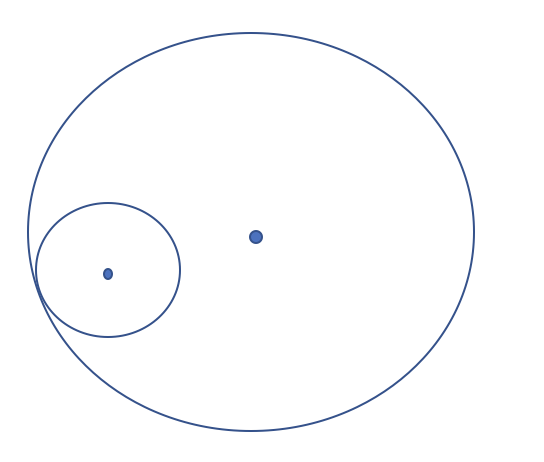
\includegraphics[width=4cm]{construction_of_contradictive_sequence}
\caption{The intuitive picture of construction of such a sequence}
\end{figure}
\paragraph{Excercise 1.5.3}$\Rightarrow$ To prove the boundeness, we already done it. The prove of closeness is the following. Because $Y$ is complete, a convergent sequence in $X$ that is Cauchy in $Y$ is convergent in $Y$. Simply put, the limit of a convergent sequence in $Y$ lies in $Y$. Therefore, it is closed.\\
$\Leftarrow$ By proposition 1.1.18, it is sufficient to only show the target statement with $(\mathbb{R}^n,d)$ be a sup norm metric. By theorem 9.1.14, for every sequence $a_{n}$ in $(\mathbb{R}^n,d)$, there exists a subsequence $b_{n1}$ that the sequence of first entry of each point in it is a convergent sequence.\\Use an instance to illustrate it this.\\
\[a_{n}=\{(1.1,1),(0,2),(1.01,3),(0,4),(1.001,5),\dots\} 
\]
\[b_{n1}=\{(1.1,1),(1.01,3),(1.001,5),\dots\}
\]
For the dimension of element in metric space $(\mathbb{R}^n,d)$ $n$ is a finite number, we can do similiar procedure --- find subsequence $b_{n2}$ of $b_{n1}$ --- on and on. Till we get $b_{nn}$ that every entry of it is convergent. Then obviously, for sup norm metric, $b_{nn}$ is convergent.$\Box$\\(Remark: hope you are not confused with the notation, the first n in $b_{nn}$ want to means it is a sequence instead a point, the second is used to index the sequence of those  sequences.---hopefully I didn't make it more confused)
\paragraph{Excercise1.5.7}
\begin{itemize}
\item[(a)]$\Rightarrow$ This has been proven before.\\
$\Leftarrow$ By definition, for any sequence in $Z$, there exists a convergent subsequence in $Y$ ($Y$ is compact). Also $Z$ is closed, the limit of this convergent sequence lies in $Z$.$\Box$
\end{itemize}

\paragraph{Excercise 1.5.8} All the statementd are trivial to prove. While it seems that there exists some further theories regarding this excercise.

\paragraph{Excercise 1.5.10} 
\begin{itemize}
\item[(a)]$X \subseteq B(x^{(1)},\varepsilon+d(x^{(1)},x^{(2)})+d(x^{(2)},x^{(3)})+\dots+d(x^{(n-1)},x^{(n)}))$
\item[(b)]\textcolor{red}{This question is tough. I haven't solved yet.} This is intuitive but hard to comprehend the hint.
\item[(c)]The big picture of the hint is clear.
\end{itemize}

\paragraph{Excercise 1.5.12}(b) When $X$ is finite, $(X,d)$ is compact. Else, it isn't.
\paragraph{Excercise 1.5.15} Assume $\cap_{\alpha\in I}K_{\alpha} = \varnothing$, then $X/\cap_{\alpha\in I}K_{\alpha}=X$. By Morgan's Law, we have $\cup_{\alpha\in I} X/K_{\alpha}=X$ $\dots$(1)\\
Because every $K_{\alpha}$ is closed, $X/K_{\alpha}$ is open. By (1) and compactness of $X$, we know that there exist finite subset $\cup(X/K_{\alpha})_{\alpha\in E}$ of $\cup(X/K_{\alpha})_{\alpha\in I}$ cover $X$. This implies a contradiction; a finite union $\cap(K_{\alpha})_{\alpha\in E}=\varnothing$.\\
Counterexample:\\$(Q,d)$ be the metric space. $K_{n}=\{x|x\in \mathbb{Q}, x\in[\sqrt{2}-\frac{1}{n},\sqrt{2}]\}$, as we can see, $\cup_{n\in\mathbb{N}}K_{n}=\varnothing$.

\begin{figure}[H]
\centering
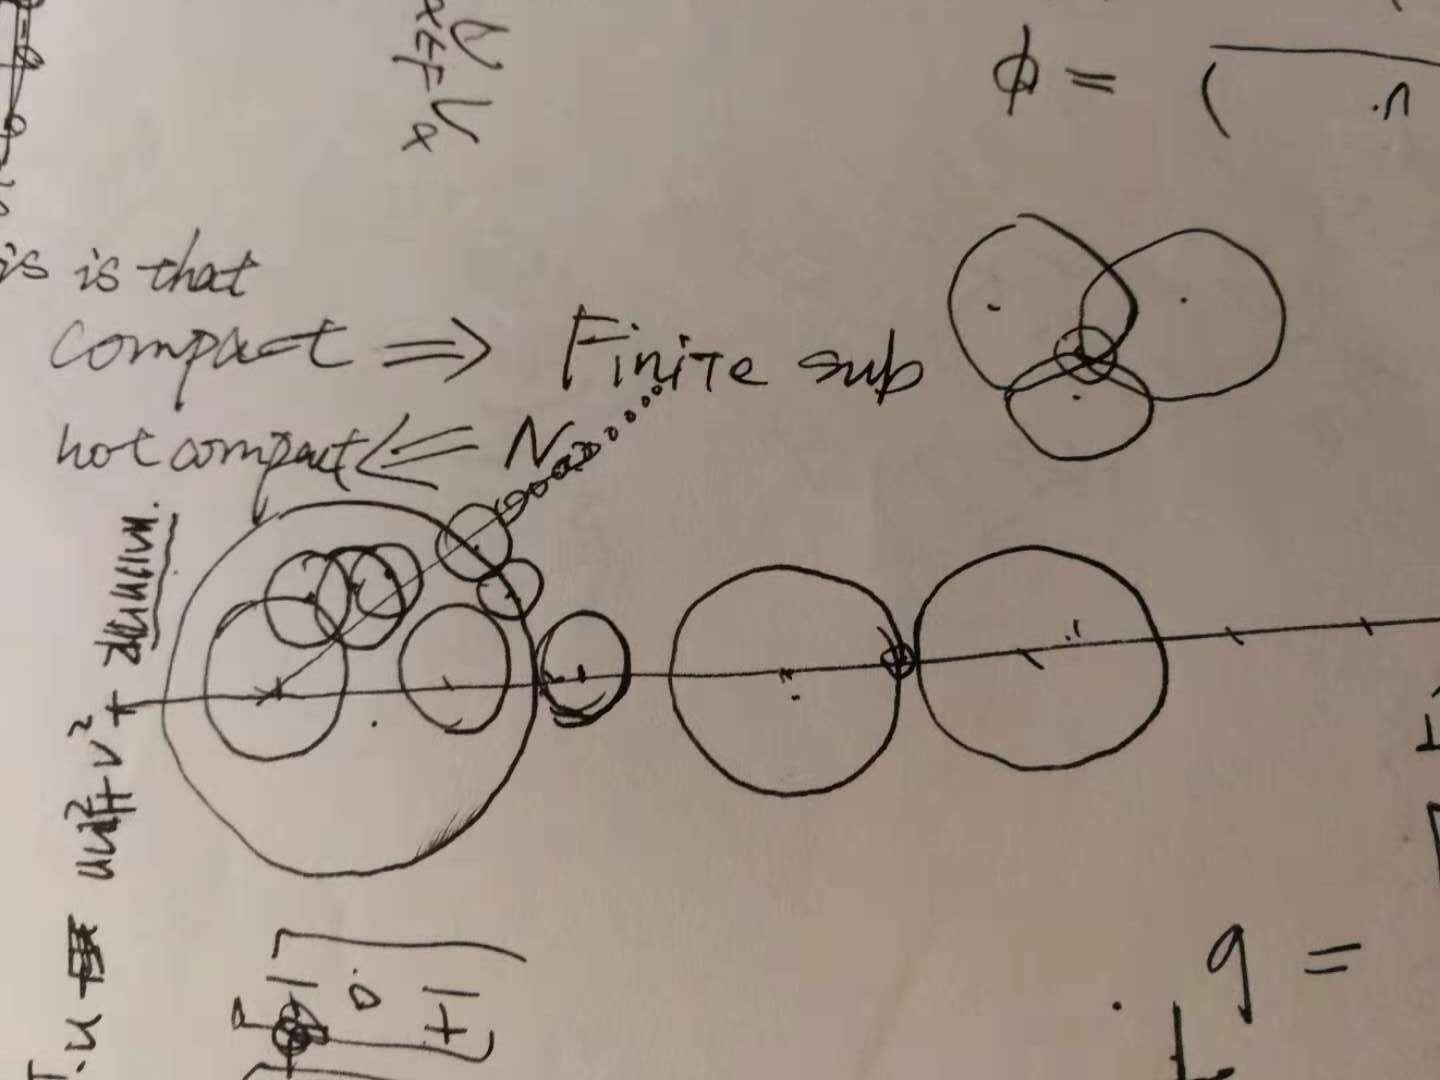
\includegraphics[width=6cm]{some_unspeakable_thoughts1.jpeg}
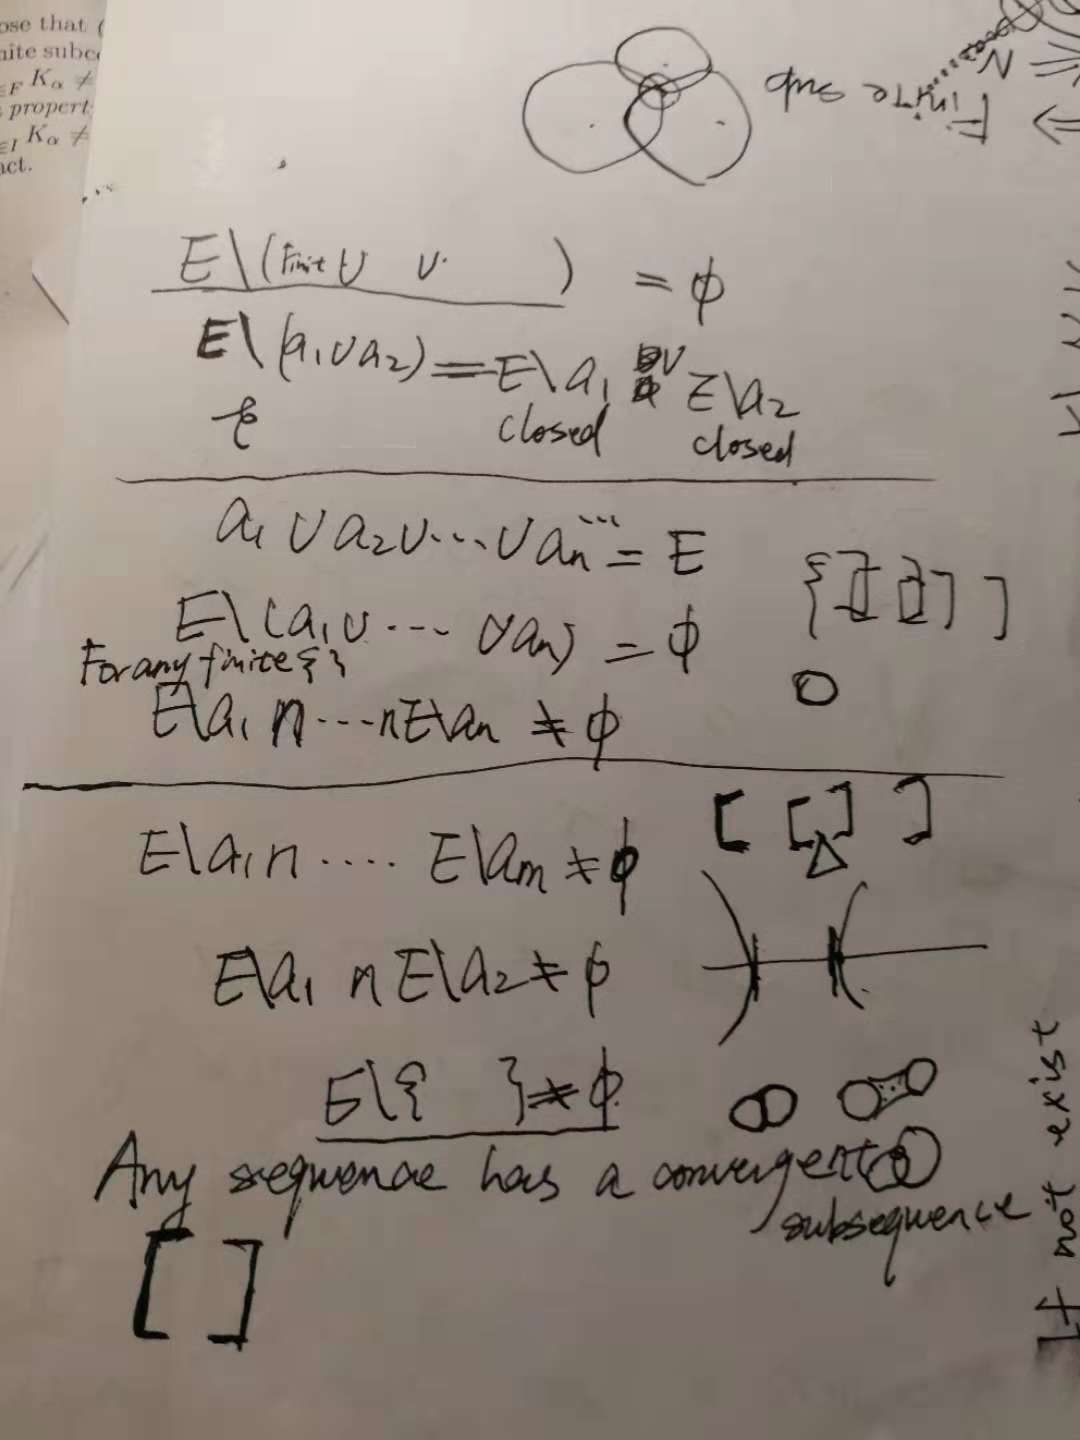
\includegraphics[width=6cm]{some_unspeakable_thoughts2.jpeg}
\caption{My primary thoughts before This excercise.}
\end{figure}






\chapter{Continuous function on metric spaces}
\section{Continuous functions}
\paragraph{Excercise 2.1.1}
\begin{itemize}
\item[(a)$\Rightarrow$(b)]Let $(x^{(n)})_{n=1}^{\infty}$ a sequence converges to $x_{0}$. For fucntion $f$ is continuous, $\forall \varepsilon$ $\exists \delta$ s.t. when $d(x_{0},x)<\delta$, $d(f(x),f(x_{0}))<\varepsilon$. For $(x^{(n)})_{n=1}^{\infty}$ converges to $x_{0}$, there exists $N$ when $n>N$, $d(x^{(n)},x_{0})<\delta$. Therefore, $d(f(x^{(n)}),f(x_{0}))<\varepsilon$ when $n>N$.
\item[(b)$\Rightarrow$(c)] Prove its conter proposition. Assume for every open set $V \subset Y$ that contains $f(x_{0})$, for any open sets $U \subset X$ containing $x_{0}$, $f(U)\nsubseteq V$ which means there exists a point $x^\prime\in U$; $f(x^\prime)\notin V$. From above, we know we can construct a sequence $a_{n}\rightarrow x_{0}$ whose $(f(x^{(n)}))_{n=1}^{\infty}$ doesn't converges to $f(x_{0})$ \Lightning. Therefore, statement does hold.
\item[(c)$\Rightarrow$(a)]
Patently.
\end{itemize}
\paragraph{Excercise 2.1.2}
\begin{itemize}
\item[(a)$\Rightarrow$(c)] Form previous excercise, we know that\\ {\it For every open set $V \subset Y$ that contains $f(x_{0})$, there exists an open set $U \subset X$ containing $x_{0}$ such that $f(U) \subset V$.}\dots(1)
\\
For a point $x^\prime$ in $f^{-1}(V)$, $f(x^\prime)$ belongs to $V$ which is open. There exists a open set $B_{r}(f(x^\prime))$ in $V$. By (1), there exists a open set $U^\prime \subset X$ containing $x^\prime$ such that $f(U^\prime) \subseteq V$. The existance of $U^\prime$ implies $f^{-1}(V)$ is open.
\item[(c)$\Rightarrow$(a)] Similiarly, prove (c) can $\Rightarrow$ (1).
\item[(c)$\Rightarrow$(d)]With proposition 1.2.5.(e), and proposition 1.3.4, it is easy to see. 
\end{itemize}
\paragraph{Excercise2.1.6}
The right direction is induced. However, the reverse direction is wrong.For example, the dilichlet function is continuous in $\mathbb{Q}$, but not in $\mathbb{R}$.
\section{Continuity and product spaces}
\paragraph{Excercise2.2.5}
\begin{proof}
From excercise 2.2.4, we know that $P_{1}(x,y)=x$ is a continuous function. By corollary 2.2.3, we know that $P_{2}(x,y)=c_{ij}x\times y$ is also continuous. By induction, we know that $P(x,y)=\sum_{i=0}^{n}\sum_{j=0}^{m}c_{if}x^{i}y^{j}$ is continuous.
\end{proof}
\paragraph{Excercise2.2.7} We have already
find that, when $k=2$, statement holds. Assume it holds for $k=n$ (\[P(x_{1},\dots,x_{n}):=\sum_{(i_{1},\dots,i_{n})\in I}c(i_{1},\dots,i_{n})x_{1}^{i_{1}}\dots x_{n}^{i_{n}}\qquad\dots(1)\] is continuous) , let's show it is also true for $k=n+1$.\\ Patently, each term of $P(x_{1},\dots,x_{n+1})$ is continuous.\dots (2) (why is that, see following)\\
Because, from (1), for any particular $(i_{1},\dots,i_{n},i_{n+1})\in I$, function $y=c(i_{1},\dots,i_{n},i_{n+1})x_{1}^{i_{1}}\dots x_{n}^{i_{n}}$ is continuous. In addition, function $y=x_{n+1}^{i_{n+1}}$ is continuous. Therefore, (2) holds with the help of limit law. For $I$ is finite, we can use corollary 2.2.3 (b) finitely many times to finish the proof.
\paragraph{Excercise2.2.8\textcolor{red}{Toberemained}} In fact, this isn't quite clear to me. However, I will have a try. The following is the analogue of proposition 1.1.18.\\
Let $X\times Y$ be the metric space that mentioned in the book, let $(x^{(k)})_{k=m}^{\infty}$ be a sequence of points in $X\times Y$. We write $x^{(k)}
=((x_{1}^{(k)},x_{2}^{(k)},\dots,x_{m}^{(k)}),(x_{1}^{(k)},x_{2}^{(k)},\dots,x_{n}^{(k)}))$, i.e., for \\
\dots, I am tired. I don't want to think it out explicitly and type it down.

\paragraph{Excercise 2.2.9}
I will only show $\lim_{x\rightarrow x_{0}}\limsup_{y\rightarrow y_{0}}f(x,y)=f(x_{0},y_{0})$
\begin{figure}[H]
\centering
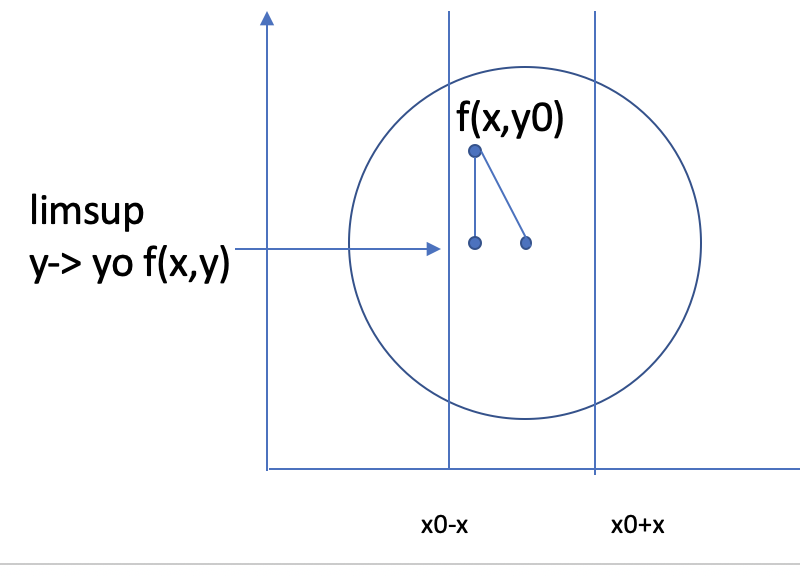
\includegraphics[width=8cm]{Excercise229}
\caption{Intuition figure}
\end{figure}
\begin{proof}
$\forall\varepsilon$ $\exists \delta$ s.t. for all $d((x,y),(x_{0},y_{0}))<\delta$, $|f(x,y)-f(x_{0},y_{0})|<\varepsilon$.\\Then for $|x^\prime-x_{0}|<\frac{\sqrt{2}\delta}{2}$, there exists $|y^\prime-y_{0}|<\frac{\sqrt{2}\delta}{2}$;
\[|f(x^\prime,y^\prime)-\limsup_{y\rightarrow y_{0}}f(x^\prime,y)|<\varepsilon\]
In addition, for $d((x^\prime,y^\prime),(x_{0},y_{0}))<\delta$,
\[|f(x^\prime,y^\prime)-f(x_{0},y_{0})|<\varepsilon
\]
Therefore,
\[|f(x_{0},y_{0})-\limsup_{y\rightarrow y_{0}}f(x^\prime,y)|<2\varepsilon
\]


\end{proof}
\section{Continuity and compactness}
\paragraph{Excercise2.3.1}
For any sequence $\{f(x_{n})\}_{n}$ in $f(K)$, there exists a convergent subsequence $\{x_{n^\prime}\}_{n^\prime}$. Then the subsequence $\{f(x_{n^\prime})\}_{n^\prime}$ of $\{f(x_{n})\}_{n}$ is convergent because of continuity of $f$.
\paragraph{Excercise2.3.2}First, want to show that: $f$ is bounded. Assuem $f$ isn't bounded, then we can construct a sequence $\{x_{n}\}_{n}$ such that it goes to infinity. Because of the compactness of $X$, there exists a convergent subsequence $\{x_{n^\prime}\}_{n^\prime}$ whose image
$\{f(x_{n^\prime})\}_{n^\prime}$ diverges. This contradict to the fact that $f$ is continuous.\\
Secondly, set the $sup(f(X))$ be a. If there exists a $x$ that $f(x)=a$, then we are done. If not, we can  which means we can construct a monotone increasing sequence $\{f(x_{n})\}_{n}\rightarrow a$. Again, for $X$ is compact, there exists a convergent subsequence $\{x_{n^\prime}\}_{n^\prime}\rightarrow x_{0}$ of $\{x_{n}\}_{n}$. $f(x_{0})=a$ because of continuity of $f$  \Lightning.
\section{Continuity and connectedness}
\paragraph{Excercise 2.4.1} For a element $x$ in $E$, then $E=\{x\}\cup (E/\{x\})$. In particular,$\{x\}$ and $(E/\{x\})$ are open set( for any point, consider those neighbourhood with radius less than $\frac{1}{2}$).
\paragraph{Excercise 2.4.3} I don't know how to show $(b)\rightarrow(c)$.
\paragraph{Excercise 2.4.6} 
\begin{proof}
Assume $f(E)$ is not connected; $f(E)=U\cup V$, where $U$ and $V$ are disjoint. For $f$ is continuous, $f^{-1}(U)$ and $f^{-1}(V)$ are open set. Then $f^{-1}(U)\cap f^{-1}(V)\neq\emptyset$ because of connectedness of $E$. For a point $x\in f^{-1}(U)\cap f^{-1}(V)$, we can see that $f(x)\in U$ and $f(x)\in V$ which is ridiculous. Therefore, $f(E)$ is connected.
\paragraph{Excercise2.4.6}For any two open set, $V$ and $W$, satisfied $U\cup W=\bigcup_{\alpha\in I}E_{\alpha}$, we want to show they are adjoint. 
\[
\bigcup_{\alpha\in I}E_{\alpha}=\{\bigcap_{\alpha\in I}E_{\alpha}\}\cup\{\bigcup_{\alpha\in I}E_{\alpha}/\bigcap_{\alpha\in I}E_{\alpha}\}
\]
w.l.o.g. assume an element $a\in\bigcap_{\alpha\in I}E_{\alpha}$ is in $W$. Then, for $V$ is non-empty, there is a element $b\in E_{\alpha^\prime}$ for $\alpha^\prime\in I$. From above, we can draw the conclusion that:$W\cap E_{\alpha^\prime}\neq\emptyset$ and $V\cap E_{\alpha^\prime}\neq\emptyset$.\\ In addition, $\{V\cap E_{\alpha^\prime}\}\cup\{W\cap E_{\alpha^\prime}\}=\{V\cup W\}\cap E_{\alpha^\prime}=\bigcup_{\alpha\in I}E_{\alpha}\cap E_{\alpha^\prime}=E_{\alpha^\prime}$\dots (1). Now, we know (1), $\{V\cap E_{\alpha^\prime}\}$ is open w.r.t. $(E_{\alpha^\prime},d_{E_{\alpha^\prime}\times E_{\alpha^\prime}})$ (so does $W$) and $E_{\alpha^\prime}$ is connected. Then $\{V\cap E_{\alpha^\prime}\}\cap\{W\cap E_{\alpha^\prime}\}\neq\emptyset$, so is $V\cap W$.
\end{proof}
\paragraph{Excercise2.4.7}For two non-empty open sets $V$, $W$ satisfied $V\cup W=E$, we pick $a\in V$ and $b\in W$. There is a conituious function $\gamma:[0,1]\rightarrow E$ such that $\gamma(0)=a,\gamma(1)=b$. Then $\gamma([0,1])$ is connected. Union of two open sets $(V\cap\gamma([0,1])) \cup (W\cap\gamma([0,1]))$ equal $\gamma([0,1])$ $(V\cap\gamma([0,1])) \cap (W\cap\gamma([0,1]))\neq\emptyset$.
Therefore, $V\cap W\neq\emptyset$. 
\paragraph{\textcolor{red}{Excercise2.4.9}} I havn't solve this question. Never mind, I'll just keep going.
\section{Topological spaces (Optional)}
\paragraph{Excercise 2.5.4}Assume $\{x^{(n)}\}_{n}$ converges to x. Then W.T.S that for any $a\neq x$, $\{x^{(n)}\}_{n}$ doesn't converge to $a$ for Hausdorff topological space. There exist two sets $U$, $W$ s.t. $x\in U$, $y\in W$ and $U\cap W=\emptyset$. Then there exists an $N$ s.t. for $n>N$, $x^{(n)}\in U$. Which means there exists a neighbourhood $W$ of $a$ such that there doesn't exist an $N$ such that $x^{(n)}\in W$ for all $n>N$.\\
Counter-example:$(X,\mathcal{F})$,$X={a,b,c}$, $\mathcal{F}=\{\{a,b,c\}\{a,b\}\{c\}\}$. Then, $a,\dots, a,\dots$ converges both a and b.
\paragraph{\textcolor{red}{Excercise 2.5.6}}


















\chapter{Uniform convergence}
\section{Limiting values of functions}
\paragraph{Excercise 3.1.1}
I still trying to comprehend those things. Those are intuitive, but details are not that clear.
\section{Pointwise and uniform convergence}
\paragraph{Excercise 3.2.1}
\begin{itemize}
\item[(a)]$\Rightarrow$ $f$ is continuous, then for a sequence $x-a_{n}$ converges to $x$. $f_{n}(x)=f(x-a_{n})\rightarrow f(x)$. Thus, it is point wise continuous.\\
$\Leftarrow$ To show $f$ is continuous that is to show for any given sequence $a_{n}$ goes to $x$, $f(a_{n})\rightarrow f(x)$.\\ Pf: For any $x$ and any given sequence $b_{n}$ goes to $x$, there exists a sequence $a_{n}$ such that $b_{n}=x-a_{n}$. $f(b_{n})=f(x-a_{n})=f_{a_{n}}(x)\rightarrow f(x)$\\
\item[(b)]$\Rightarrow$ $\forall\varepsilon$ there exists a $\delta$ s.t. $d(f(x),f(y))<\varepsilon$ when $d(x,y)<\delta$  ($f$ is uniformly continuous.). Then there exists $N$, s.t. $d(x,x-a_{n})<\delta$, when $n>N$. This implies $d(f(x),f(x-a_{n}))<\varepsilon$. This is the same as $d(f^{(n)}(x),f(x))<\varepsilon$.$\Box$\\
$\Leftarrow$ Assume this isn't the case, which means; when the shifted functions $f_{a_{n}}$ converge uniformly to $f$, $f$ isn't uniformly continuous. Then there exists a $\varepsilon>0$ s.t. , for any $\frac{1}{n}$, there exist $x_{n}$, $y_{n}$, satisfies $d(x_{n},y_{n})<\frac{1}{n}$, $d(f(x_{n}),f(y_{n}))>\varepsilon$. We set $a_{n}:=x_{n}-y_{n}\rightarrow 0$. $f_{a_{n}}$ is not converge uniformly to $f$ (why?).\Lightning$\Box$\\

\end{itemize}

\paragraph{Excercise 3.2.4} $f_{n}$ converges uniformly to $f$. Then there exists a $N$ such that, for all $n>N$ and arbitrary $x$, $d(f(x),f_{n}(x))<R$ (The $R$ for $f(x)$.). This implies there is only a need for considering those $f_{n}$ with $n<N$. Because all those $f_{n}$ ($n<N$) is bounded uniformly, there exist finitely many balls $B_{(Y,d_{Y})}(y_{m},R_{m})$ that cover $f_{n}$ respectively. Intently, $B_{Y,d_{Y}}(y_{0},R_{0})$ with $R_{0}:=max\{d(y_{m},y_{0})\}+max\{R_{m}\}+R$ is the ball that shows that $f_{n}$ is bounded uniformly.

\section{Uniform convergence and  ontinuity}
\paragraph{Excercise3.3.1} To show it is also continuous is the same as to show: for any $\varepsilon$, there exists a $\delta$ such that $d(f(x),f(x_{0}))<\varepsilon$ for all $x$ satisfies $d(x,x_{0})<\delta$--- we want to figure out the $\delta$. \\
There are three $\frac{\varepsilon}{3}$ we need to satisfy. The first and last we can use uniform convergent property to satisfied; there exists a $N$ such that $d(f(x),f^{(n)}(x))<\frac{\varepsilon}{3}$, for all $x$ and $n>N$. Then we can pick a particular $n_{0}=N+1$. For $f^{n_{0}}$ is contiunous at $x_{0}$, there exists a $\delta_{0}$ to make the middle $\frac{\varepsilon}{3}$ hold.$\Box$
\paragraph{Excercise3.3.2}
With the help of proposition3.1.5, first we need to show that $\lim_{x\rightarrow x_{0};x\in E}f(x)$ exists in the sequence point of view.\\
For any $x_{n}\rightarrow x$, $x_{n}\in E$, we want to show that $\{f(x_{n})\}_{n}$ is Cauchy ( $Y$ is complete.). This is the same as to show that: there exists $N_{0}$ such that $d_{Y,d_{Y}}(f(x_{n}),f(x_{m}))<\varepsilon$ when $n,m>N_{0}$.
\[d_{Y,d_{Y}}(f(x_{n}),f(x_{m}))<d_{Y,d_{Y}}(f(x_{n}),f^{p}(x_{n}))+d_{Y,d_{Y}}(f^{p}(x_{n}),f^{p}(x_{m}))+d_{Y,d_{Y}}(f^{p}(x_{m}),f(x_{m}))
\]
Like previous excercise, pick particular $p$. Then we can get the $N_{0}$ we want.
This means $\{f(x_{n})\}_{n}$ is indeed Cauchy (convergent). Therefore, $\lim_{x\rightarrow x_{0};x\in E}f(x)$ is meaningful.\\
\\
Secondly, we want to show that $\lim_{n\rightarrow\infty}\lim_{x\rightarrow x_{0};x\in E}f^{(n)}(x)$ converges to $\lim_{x\rightarrow x_{0};x\in E}f(x)$; $\forall\varepsilon$ $\exists N_{0}$, when $n>N_{0}$,
$d_{Y,d_{Y}}(\lim_{x\rightarrow x_{0},x\in E}f(x),\lim_{x\rightarrow x_{0},x\in E}f^{(n)}(x))<\varepsilon$.\dots (1)\\
For a sequence $x_{m}$ converges to $x$, there exists $N=max\{N_{1},N_{2}\}$ make \\$d_{Y,d_{Y}}(f(x_{m}),\lim_{x\rightarrow x_{0},x\in E}f(x))<\frac{\varepsilon}{3}$ and $d_{Y,d_{Y}}(f^{(n)}(x_{m}),\lim_{x\rightarrow x_{0},x\in E}f^{(n)}(x))<\frac{\varepsilon}{3}$ when $m>N$.
At $x_{m}$, of course, there exists $N_{0}$ s.t. $d_{Y,d_{Y}}(f(x_{m}),f^{(n)}(x_{m}))$ when $n>N_{0}$. We have already found the target $N_{0}$ and, with the help of triangular inequality, (1) is true.$\Box$

\paragraph{Excercise3.3.8}
\[|f_{n}g_{n}-f_{n}g+f_{n}g-fg|\leq|f_{n}||g_{n}-g|+|g_{n}||f_{n}-f|
\]










\chapter{Several variable differential calculus}
\section{Linear transformation}
\paragraph{Excercise 6.1.43.}
\begin{proof}
\[(L_{AB}x)\trans=ABx\trans=A(L_{B}x)\trans=(L_{A}(L_{B}x))\trans
\]
Hence, $L_{A}L_{B}=L_{AB}$
\end{proof}
\section{Derivatives in several variable caculus}
\paragraph{Excercise 6.2.1.}
\begin{proof}With a little bit arrangement, the following inequality can be got.
\[\|\frac{f(x_{0}+tv)-f(x_{0})}{t}-L_{1}(v)\|<\varepsilon\]
\[\|\frac{f(x_{0}+tv)-f(x_{0})}{t}-L_{2}(v)\|<\varepsilon\]
\begin{figure}[H]
\centering
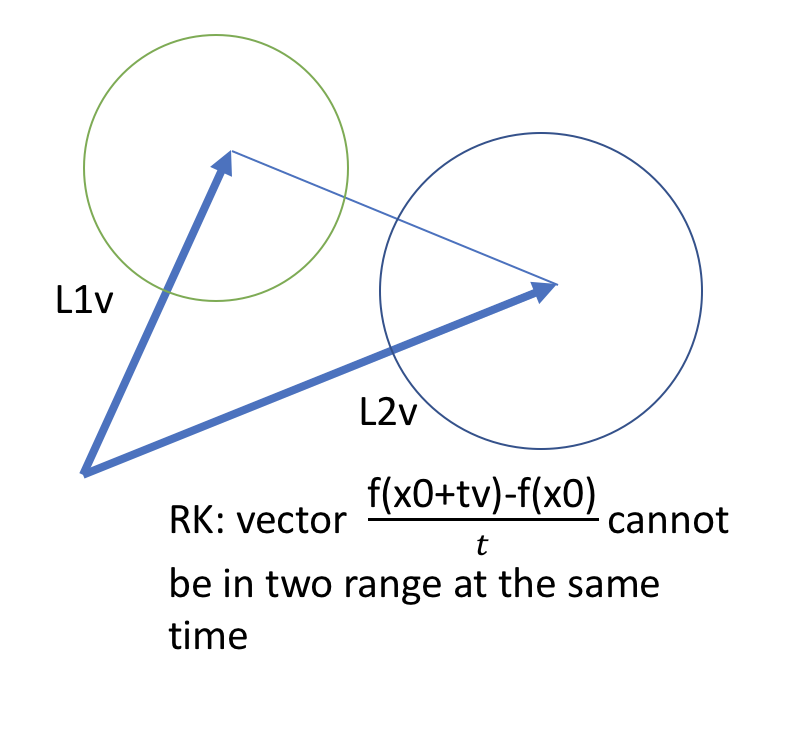
\includegraphics[width=8cm]{Uniqueness_Of_Derivatives}
\caption{Range of vector $\frac{f(x_{0}+tv)-f(x_{0})}{t}$}
\end{figure}
Pick $\varepsilon$ careful enough($<\|\frac{L_{1}(v)-L_{2}(v)}{2}\|$), we can make the contradiction.
\end{proof}
\section{Partial and directional derivatives}
\paragraph{6.3.3.}The big idea is that the partial derivatives all exists at (0,0) but it isn't continuous at (0,0). Also, it is not differentiable at(0,0).
Take partial derivative of second variable as an example. It is easy to check that $\frac{\partial f}{\partial y}(0,0)=0$
\begin{align}
\frac{\partial f}{\partial y}(t_{1},t_{2})&=\lim_{t\rightarrow 0}\frac{f(t_{1},t_{2}+t)-f(t_{1},t_{2})}{t}
\\&=\lim_{t\rightarrow 0}\frac{t_{1}^3}{(t_{1}^2+t_{2}^2)}\frac{(-2t-2t_{2})}{(t_{1}+t_{2}^2+4tt_{2}+3t^2)}\\
&=\frac{-2t_{1}^3t_{2}}{(t_{1}^2+t_{2}^2)^2}
\end{align}
When $t_{1}=t_{2}$ and they both go to zero,
\[\lim_{(t_{1},t_{2})\rightarrow (0,0)}\frac{\partial f}{\partial y}(t_{1},t_{2})=-\frac{1}{2}\neq0\]
From above, it is clear that the partial derivative exists but not continuous. Therefore, it doesn't contradict Theorem 6.3.8. I think $\frac{\partial f}{\partial x}$ is something similiar which is left to readers. (While, I haven't done it.)\\Now let's prove why it is not differentiable.
\begin{proof}
We want to show for any Linear transformation $L$. There exists a $\varepsilon$ s.t. for any $\delta$ there exists a point near (0,0) within $\delta$ (which is to say $\sqrt{x^2+y^2}\leq\delta$) satisfies:
\[\frac{\|f(x,y)-f(0,0)-L(x,y)\|}{\|(x,y)\|}>\varepsilon
\]
which is same as to prove there always exists (x,y) s.t.
\[|\frac{x^3}{x^2+y^2}\frac{1}{\sqrt{x^2+y^2}}-\frac{A(x,y)\trans}{\sqrt{x^2+y^2}}|>\varepsilon
\]
(Linear transformation $L$ is equivalent to matrix $A=(a,b)$)
\[|(\frac{x}{\sqrt{x^2+y^2}})^3-\frac{(a,b)(x,y)\trans}{\sqrt{x^2+y^2}}|>\varepsilon
\]
\[|cos(\alpha)^3-acos(\alpha)-bsin(\alpha)|>\varepsilon
\]
With the change of variable, it is more clear that for any given $a, b$ there exist a $cos(\alpha)$ to hold the inequality ( with $\|(x,y)\|<\delta$). Although the proof is not that rigorous for we didn't find the $\varepsilon$, this is more intuitively than before.
\end{proof}
\paragraph{\textcolor{red}{Excercise 6.3.4.}} Maybe we should treat component of function $f$ seperately. After constructing a function $\phi_{1}(t): \mathbb{R}\rightarrow\mathbb{R} := f_{1}(x+t(x^\prime-x))$, we can use MVT. To show that $f_{1}(x)=f_{1}(x^\prime)$. When the domain $\mathbb{R}^n$ is replaced by an open connected subset $\Omega$ of $\mathbb{R}^n$, I didn't see any differences.

\section{The several variable calculus chain rule}
\paragraph{Excercise 6.4.1} Let $A$ be the matrix representation of linear transformation $T$. $T^\prime=A$
The reason is:
\[\|Ax-A_{x_{0}}-A(x-x_{0})\|=0<\varepsilon
\]
Also $DT=A$
\paragraph{Excercise 6.4.2} A function $f$ is differentiable at $x_{0}$, then there exist a \emph{linear transformation} $f^\prime(x_{0})$ satisfies the following:
\[\|f(x)-f(x_{0})\|\leq\|f(x)-f(x_{0})-f^\prime(x_{0})(x-x_{0})\|+\|f^\prime(x_{0})(x-x_{0})\|\leq\varepsilon\|x-x_{0}\|+M\|x-x_{0}\|
\]
The inequality of right hand side is because of excercise6.1.4.
Because of the inequality, indeed, it is continuous.
\paragraph{Excercise 6.4.3}\begin{proof}Clarification:\\
The goal is to show that every sequence which converges to $x_{0}$ has the property that:
\[\lim_{x\rightarrow x_{0}}\frac{\|(g\circ f)(x)-(g\circ f)(x_{0})-g^\prime(f(x_{0}))f^\prime(x_{0})(x-x_{0})\|}{\|x-x_{0}\|}=0
\]
What we have is function $g$ is differentiable at $f(x_{0})$ which means:
\begin{equation}\label{a}
\lim_{y\rightarrow f(x_{0})}\frac{\|g(y)-g(f(x_{0}))-g^\prime(f(x_{0}))(y-f(x_{0}))\|}{\|y-f(x_{0})\|}
\end{equation}
Also, fucntion $f$ is differentiable at $x_{0}$:
\begin{equation}\label{b}
\lim_{x\rightarrow x_{0}}\frac{\|f(x)-f(x_{0})-f^\prime(x_{0})(x-x_{0})\|}{\|x-x_{0}\|}
\end{equation}
When $x\rightarrow x_{0}; f(x)\rightarrow f(x_{0})$, by excercise 6.4.2. Therefore, \ref{b} can be expressed as:
\[\lim_{x\rightarrow x_{0}}\frac{\|g(f(x))-g(f(x_{0}))-g^\prime(f(x_{0}))(f(x)-f(x_{0}))\|}{\|f(x)-f(x_{0})\|}=0
\]
%Let's say it is $a_{1}=\lim_{x\rightarrow x_{0}}\frac{\|g(f(x))-g(f(x_{0}))-g^\prime(f(x_{0}))(f(x)-f(x_{0}))\|}{\|f(x)-f(x_{0})\|}=0$ for short.\\
From excercise 6.4.2. we know that $\exists$ constant $M$ s.t. $\|f(x)-f(x_{0})\|<M\|x-x_{0}\|$\\
Therefore,
\begin{equation}\label{d}\lim_{x\rightarrow x_{0}}\frac{\|g(f(x))-g(f(x_{0}))-g^\prime(f(x_{0}))(f(x)-f(x_{0}))\|}{\|x-x_{0}\|}=0
\end{equation}
With \ref{a}, we can get
\begin{align}
0\leq&\label{c}\lim_{x\rightarrow x_{0}}\frac{\|-g^\prime(f(x_{0}))f^\prime(x_{0})(x-x_{0})+g^\prime(f(x_{0}))(f(x)-f(x_{0}))\|}{\|x-x_{0}\|}\\\\
\leq&\lim_{x\rightarrow x_{0}}\frac{\|g^\prime((f(x_{0}))(f(x)-f(x_{0})-f^\prime(x_{0})(x-x_{0}))\|}{\|x-x_{0}\|}\\\\
\leq&\lim_{x\rightarrow x_{0}}\frac{\|g^\prime((f(x_{0}))\|\|f(x)-f(x_{0})-f^\prime(x_{0})(x-x_{0})\|}{\|x-x_{0}\|}=0
\end{align}
Add \ref{c} to \ref{d}, we get the target.
\end{proof}








\backmatter

\latexprintindex

\end{document} 